\section*{Summary of the Proposal}

\textit{Aheui}~\cite{aheui} is the first esoteric programming language ever to be designed for the Hangul(Hangeul) . The aim of the language is to reflect the graphical design of Hangul. Aheui has no practicality at all, but it is a language that is often talked about in the Korean developer community because of its visual characteristics. Based on such pure interest, there are many works that have implemented Aheui of various interpreter behaviors. However, no work has been done in compiled form. This project focuses on making Aheui a compilable language on \textit{LLVM}. This work will be done on Aheui's language specification, \textit{Flex}, \textit{Bison}, and \textit{LLVM}. Therefore, the result of this work will be able to use existing functions and advantages of \textit{LLVM} such as machine-independence and common IR optimizer. I just hope that this project will become a kind of another fun story for the Korean developer community.

\section*{Background}

\textit{Aheui} is the first esoteric programming language ever to be designed for the Hangul (Hangeul) . The aim of the language is to reflect the graphical design of Hangul. The aim of the language is to reflect the graphical design of Hangul. Aheui is a stack-based programming language that works in a similar fashion to Befunge / Funge-98, but it differs in that it is Hangul, not ASCII. Note that Befunge has \textit{p} and \textit{q} commends to generate self-modifying code because it was originally presented as a "language that is hard to compile" for research purposes, but Aheui has no such commend. The code for outputting the most famous program, "Hello, world!", Looks like this:
\\
\begin{figure}[ht!]
\centering
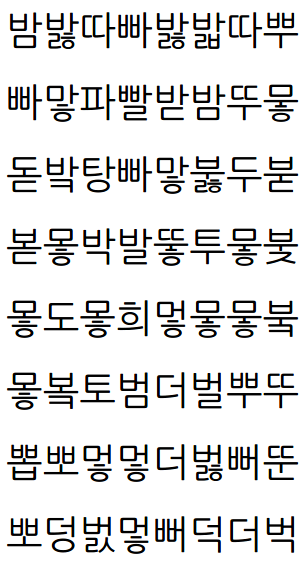
\includegraphics[width=20mm]{helloworld.png}
\caption{A simple "Hello, world!" program in \textit{Aheui}\label{overflow}}
\end{figure}

Due to the interestingness of the language so far, the following tasks related to its implementation have been found.

\begin{itemize}
\item Interpreter implementations by other languages or runtime environments~\cite{aheui_projects} such as Ruby, Scala, ActionScript, Rust, Python, PyPy, JavaScript, C, Node.js, and Go. In particular, \textit{Rpaheui}, an interpreter implemented by PyPy, is a JIT interpreter.
\item Works for visualization of Aheui code execution : \textit{AVIS}~\cite{avis}, \textit{AheuiChem}~\cite{aheuichem}
\item An alternate implementation of the \textit{Aheui} programming language written in \textit{Aheui}, called \textit{aheui.aheui}~\cite{aheuiaheui}
\end{itemize}

Although \textit{Rpaheui} introduced an asembly-like code generator for code linearization, it was not code that could be used as an ISA. In conclusion, there is no work that essentially transforms the Aheui program for optimization or profiling. On the other hand, in the case of Befunge, which is inevitably more difficult to create a compiler, there are \textit{bef2c} transpilers included in standard Befunge-93.

\section*{Goal and Objectives}

This project focuses on making Aheui a compilable language on \textit{LLVM}. It is possible to compare the performance of the proposed compiler with the other by comparing some of the references that run \textit{aheui.aheui} on different implementations of \textit{Aheui}. It is also possible to measure the speed of operation for several snippets.

\section*{Methods}

This work will be done on Aheui's language specification, \textit{Flex}~\cite{lesk1975lex}, \textit{Bison}~\cite{aaby2003compiler}, and \textit{LLVM}~\cite{lattner2004llvm}. All backend layers under the optimizer will be replaced by the core structure of \textit{LLVM}, and I would like to use \textit{Lex} and \textit{Bison} in frontend design rather than using \textit{LLVM} internal tools. 
\\
\begin{itemize}
\item \textit{Flex} is a tool for generating scanners, programs which recognize lexical patterns in text. Lexical analysis is easy to be done with \textit{Flex}.
\item \textit{Bison} is a general-purpose parser generator that converts an annotated context-free grammar into a deterministic LR or generalized LR (GLR) parser employing LALR parser tables. At this stage, the AST must be carefully designed.
\item \textit{LLVM} is designed for compile-time, link-time, run-time, and idle-time optimization of programs written in arbitrary programming languages. \textit{LLVM} naturally takes the AST and turn it into machine code because it abstracts the actual instructions to something that is similar to an AST. Some opimization can be done in this step.
\end{itemize}
